\section{Technical Validation Strategy}\label{ch3-sec:technical_validation_strategy}

In this section, we will discuss the technical strategy that we will adopt to tackle the scenarios and use cases mentioned in~\autoref{ch3:validation_roadmap}.

\subsection{Effective Methods to Identify Contributors, Top Contributors, and Recent Contributors}

The scenarios starting from 1 to 5, related to the authors/contributors, are merged in this section to avoid repetition since all of them require a similar approach. There are several ways to find the contributors list, author relation, top contributors, and most recent contributors:
\begin{itemize}
    \item Reviewing communication records for recent discussions or code reviews about the method. However, this process is slow and often leads to inconsistent results.
    \item Checking pull request histories on GitHub, where reviewers and contributors are listed. For repositories with many pull requests, filtering relevant changes can be overwhelming.
    \item Analyzing the repository's commit history directly from platforms like GitHub or Bitbucket. Commit messages often do not clearly indicate which methods were changed, making this process extremely time-consuming.
    \item Using the GitHub API to programmatically extract and analyze contributors' data related to specific files. However, API usage may be restricted by rate limits, especially for large repositories.
    \item Using CI/CD tools like Jenkins to monitor and report code changes and associate them with contributors. This can slow down CI/CD pipelines and requires initial setup and ongoing maintenance.
    \item Checking project documentation and looking for change logs that might include information about recent changes and contributions. However, change logs are not always updated regularly, which can lead to inaccurate results.
\end{itemize}

One of the most effective ways to achieve this is by using a version control system. In almost every project, some form of version control is used, as it allows tracking the author of the most recent changes to specific lines of code. Each project typically includes a version control file. In our test project, a \texttt{.git} directory is available, which we can parse to retrieve the required information. To achieve this, we will develop a few probes to perform static code analysis, parse the \texttt{.git} directory, and extract the necessary data to feed it into the SST. The implementation of these probes will be discussed in later chapters.

\begin{figure}[H]
    \centering
    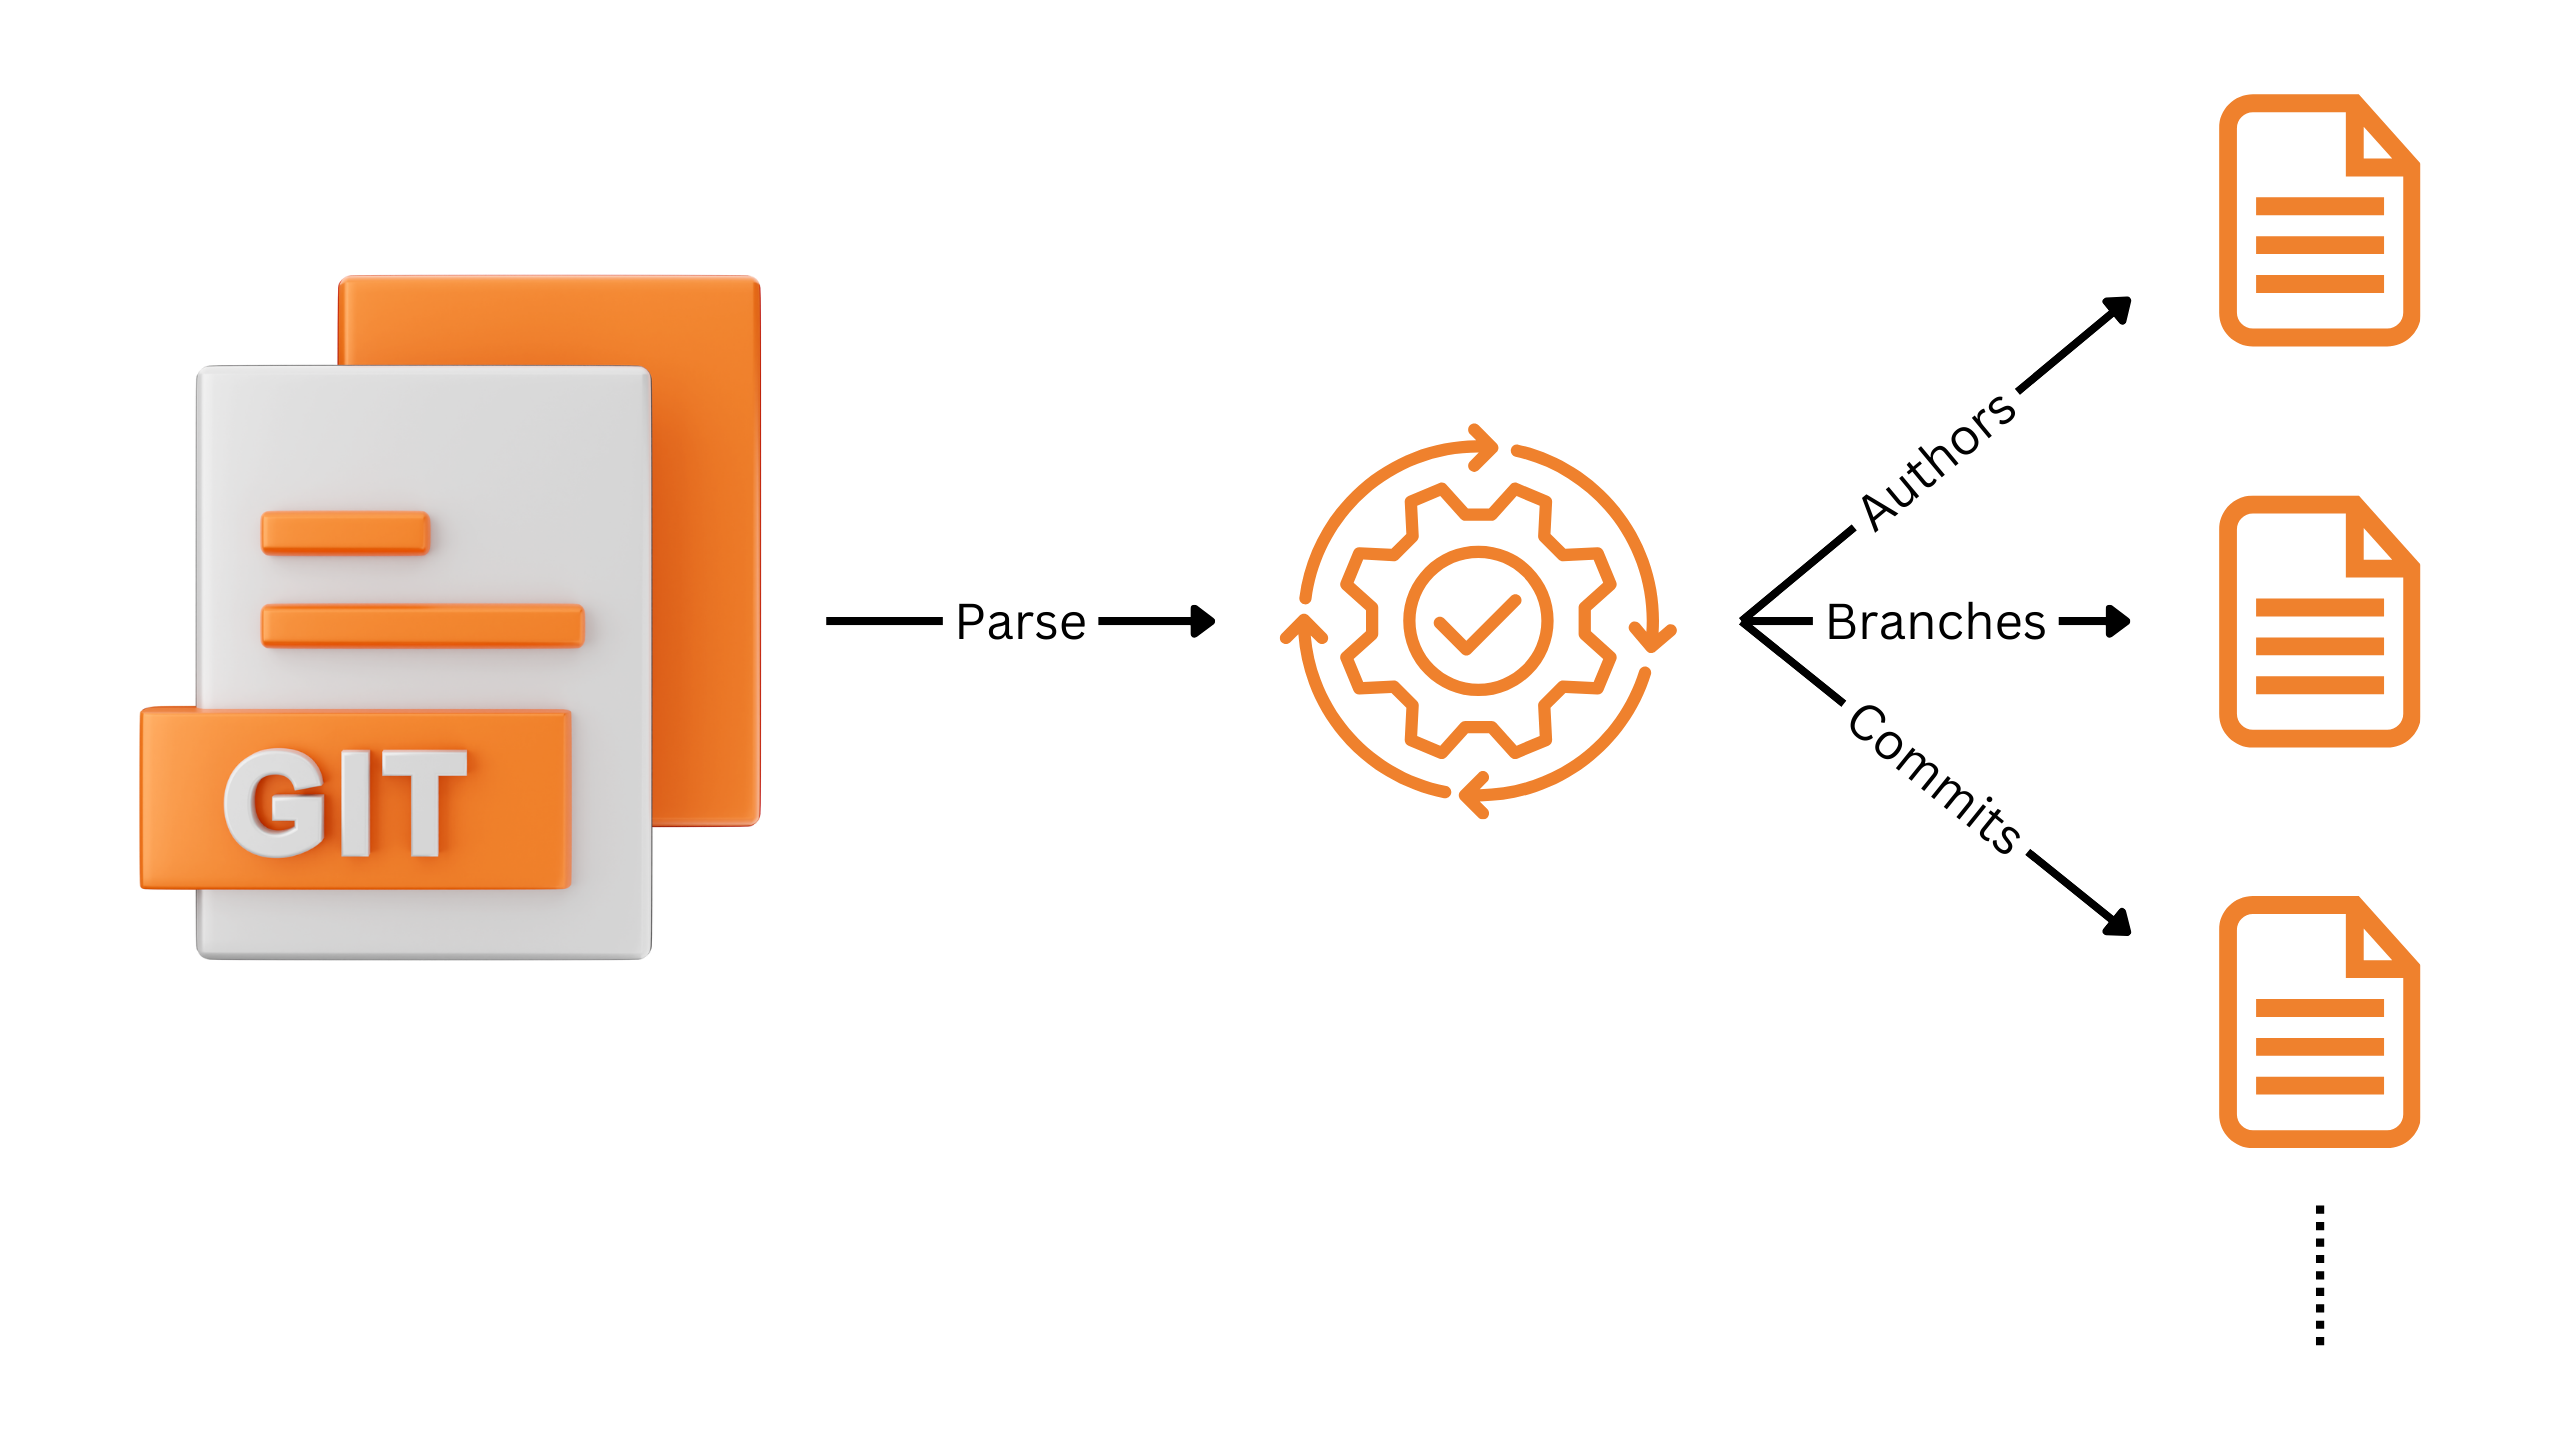
\includegraphics[width=0.8\textwidth]{figures/parse_git_file.png}
    \caption{Git Parsing Process}
    \label{fig_parse_git_file}
\end{figure}
 
\subsection{Microservices Endpoints}

For the 6th scenario, we have to determine the endpoints. \textit{REST API} endpoints for microservices can be identified in several ways from the source code. Our goal is to establish a general method for obtaining this information from your project, as real-world microservice architectures do not always use frameworks like Java Spring, as seen in the Petclinic test project referenced in this report. Below are some approaches to discovering endpoints:

\begin{itemize}
    \item Integrating Swagger\footnote{\url{https://swagger.io/}} or OpenAPI\footnote{\url{https://openai.com/}} to auto-generate documentation can be effective but requires accurate configuration for all endpoints. Misconfiguration can lead to incorrect results.
    \item Enabling logging of all incoming requests to capture and log accessed endpoints at runtime can also work. However, this approach introduces performance overhead and may miss endpoints that are rarely accessed or currently unused.
    \item Spring Boot Actuator provides an endpoint mapping system, but it only works for services based on the Spring framework.
\end{itemize}

The approach we will use involves static code analysis. We will write a probe to search for \texttt{@RequestMapping}, \texttt{@GetMapping}, \texttt{@PostMapping}, and similar annotations in the source code to identify endpoints. This probe can be configured to match the target service setup and extract REST API endpoints, which will then be stored in a unified data source.

\subsection{Beans And Dependencies}

For the 7th and 8th scenarios, We have to extract beans and dependencies from the source code. There are several ways to identify the beans and dependencies in the Spring framework project under discussion, allowing us to visualize this data for better documentation and understanding:

\begin{itemize}
    \item Spring Boot Actuator provides a \texttt{/actuator/beans} endpoint that lists all beans in the application context, along with their dependencies and initialization details. However, this can cause performance issues in large applications with many beans.
    \item The Spring \textit{ApplicationContext} can be accessed programmatically to retrieve a list of all beans and their dependencies \citep{baeldung_applicationcontext}. However, this approach requires adding custom code for bean inspection, which can increase the codebase size and potentially clutter production logs.
\end{itemize}

The approach we will use involves static code analysis. We will develop a probe to search for annotations like \texttt{@Bean}, \texttt{@Component}, \texttt{@Service}, \texttt{@Repository}, and other dependency-related annotations. Additionally, we will parse the \texttt{POM.xml} files of the services to identify the dependencies associated with each service.

\subsection{SST and Visualizer Integration}

For the 9th and 10th scenarios, integration of probes with SST and SST with visualizer is required. After extracting the necessary information, we need to demonstrate the complete capabilities of our framework by applying it to the technical scenarios we have designed. To achieve this, it is essential to integrate the extracted data with the SST with the help of REST API endpoints provided by the SST tool. Once probes and SST start exchanging data, our next task is to connect at least one visualizer tool with the SST. For that, we will connect a visualizer tool with the SST's database to obtain real-time data and information directly from the database.

The following chapter will discuss details about how the probes are integrated with SST and visualizer.
